\lab{Unit Testing}{Unit Testing}
\label{lab:PythonEssentials:UnitTesting}
\objective{
Finding and fixing programming errors can be difficult and time consuming, especially in large or complex programs.
\emph{Unit testing} is a formal strategy for finding and eliminating errors quickly as a program is constructed and for ensuring that the program still works whenever it is modified.
A single unit test checks a small piece code (usually a function or class method) for correctness, independent of the rest of the program.
A well-written collection of unit tests can ensure that every unit of code functions as intended, thereby certifying that the program is correct.
In this lab, we learn to write unit tests in Python and practice test-driven development.
Applying these principles will greatly speed up the coding process and improve your code quality.
}

% When a program contains a bug, it is easy to identify which part of the code the problem came from since only certain unit tests will fail.
% Unit Testing is extremely vital for large complex programs, especially if several people are working on the same project.
% By keeping a collection of unit tests associated with a program, developers can ensure that a program still runs correctly after modifying part of the code.

\section*{Unit Tests} % =======================================================

A \emph{unit test} verifies a piece of code by running a series of test cases and comparing actual outputs with expected outputs.
Each test case is usually checked with an \li{assert} statement, a shortcut for raising an \li{AssertionError} with an optional error message if a boolean statement is false.

\begin{lstlisting}
# Store the result of a boolean expression in a variable.
>>> result = str(5)=='5'

# Check the result, raising an error if it is false.
>>> if result is False:
...     raise AssertionError("incorrect result")

# Do the same check in one line with an assert statement.
>>> assert result, "incorrect result"

# Asserting a false statement raises an AssertionError.
>>> assert 5=='5', "5 is not a string"
<<Traceback (most recent call last):
  File "<stdin>", line 4, in <module>
AssertionError: 5 is not a string>>
\end{lstlisting}

Now suppose we wanted to test a simple \li{add()} function, located in the file \texttt{specs.py}.

\begin{lstlisting}
# specs.py

def add(a, b):
    """Add two numbers."""
    return a + b
\end{lstlisting}

In a corresponding file called \texttt{test\_specs.py}, which should contain all of the unit tests for the code in \texttt{specs.py}, we write a unit test called \li{test_add()} to verify the \li{add()} function.

\begin{lstlisting}
# test_specs.py
import specs

def test_add():
    assert specs.add(1, 3) == 4, "failed on positive integers"
    assert specs.add(-5, -7) == -12, "failed on negative integers"
    assert specs.add(-6, 14) == 8
\end{lstlisting}

In this case, running \li{test_add()} raises no errors since all three test cases pass.
Unit test functions don't need to return anything, but they should raise an exception if a test case fails.

\begin{info} % Black box testing
This style of external testing---checking that certain inputs result in certain outputs---is called \emph{black box testing}.
The actual structure of the code is not considered, but what it produces is thoroughly examined.
% Black box tests can (and should) be written \textbf{before} actually implementing a program, immediately after its specifications are defined.
In fact, the author of a black box test doesn't even need to be the person who eventually writes the program: having one person write tests and another write the code helps detect problems that one developer or the other may not have caught individually.
\end{info}

\section*{PyTest} % ===========================================================

Python's \li{pytest} module\footnote{Pytest is not part of the standard libray, but it is included in Anaconda's Python distribution. Install pytest with \li[basicstyle=\footnotesize\ttfamily]{conda install pytest} if needed. The standard library's \li[basicstyle=\footnotesize\ttfamily]{unittest} module also provides a testing framework, but is less popular and straightforward than PyTest.} provides tools for building tests, running tests, and providing detailed information about the results.
To begin, run \li{py.test} in the current directory.
Without any test files, the output should be similar to the following.

\begin{lstlisting}
$ py.test
<b<============================= test session starts =============================>b>
<<platform darwin -- Python 3.6.0, pytest-3.0.5, py-1.4.32, pluggy-0.4.0
rootdir: /Users/Student, inifile:>>
<b<collected 0 items>b>

<<========================= no tests ran in 0.02 seconds ========================>>
\end{lstlisting}

Given some test files, say \texttt{test\_calendar.py} and \texttt{test\_google.py}, the output of \li{py.test} identifies failed tests and provides details on why they failed.

\begin{lstlisting}
$ py.test
<b<============================= test session starts =============================>b>
<<platform darwin -- Python 3.6.0, pytest-3.0.5, py-1.4.32, pluggy-0.4.0
rootdir: /Users/Student/example_tests, inifile:>>
<b<collected 12 items>b>

<<test_calendar.py ........
test_google.py .F..>>

================================== FAILURES ===================================
<r<________________________________ test_subtract ________________________________>r>

    <b<def test_subtract():
>       assert google.subtract(42, 17)==25, "subtract() failed for a > b > 0">b>
<r<E       AssertionError: subtract() failed for a > b > 0
E       assert 35 == 25
E        +  where 35 = <function subtract at 0x102d4eb90>(42, 17)
E        +    where <function subtract at 0x102d4eb90> = google.subtract>r>

test_google.py:11: AssertionError
<r<===================== 1 failed, 11 passed in 0.02 seconds =====================>r>
\end{lstlisting}

Each dot represents a passed test and each \li{F} represents a failed test. % (one that raised an exception).
They show up in order, so in the example above, only the second of four tests in \texttt{test\_google.py} failed.

\begin{warn} % Naming test files and test functions with the word 'test'.
PyTest will not find or run tests if they are not contained in files named \texttt{test\_*.py} or \texttt{*\_test.py}, where \texttt{*} represents any number of characters.
In addition, the unit tests themselves must be named \li{test_*()} or \li{*_test()}.
If you need to change this behavior, consult the documentation at \url{http://pytest.org/latest/example/pythoncollection.html}.
\end{warn}

\begin{problem} % Simple unit test.
The following function contains a subtle but important error.
\begin{lstlisting}
def smallest_factor(n):
    """Return the smallest prime factor of the positive integer n."""
    if n == 1: return 1
    for i in range(2, int(n**.5)):
        if n % i == 0: return i
    return n
\end{lstlisting}
Write a unit test for this function, including test cases that you suspect might uncover the error (what are the edge cases for this function?).
Use \li{pytest} to run your unit test and discover a test case that fails, then use this information to correct the function.
\label{prob:unittest_intro}
\end{problem}

\subsection*{Coverage} % ------------------------------------------------------

Successful unit tests include enough test cases to test the entire program.
\emph{Coverage} refers the number of lines of code that are executed by at least one test case.
% Think of a function in the form of a diagram, containing branches and loops.
% Each test takes a certain path through the function, traversing some branches and not others.
% Full coverage is reached when each branch of the function is traversed by at least one test case.
One tool for measuring coverage is called \li{pytest-cov}, an extension of \li{pytest}.
This tool must be installed separately, as it does not come bundled with Anaconda.

\begin{lstlisting}[language=bash]
$ conda install pytest-cov
\end{lstlisting}

Add the flag \li{--cov} to the \li{py.test} command to print out code coverage information.
Running \li{py.test --cov} in the same directory as \texttt{specs.py} and \texttt{test\_specs.py} yields the following output.

\begin{lstlisting}
$ py.test --cov
<b<============================= test session starts =============================>b>
<<platform darwin -- Python 3.6.0, pytest-3.0.5, py-1.4.32, pluggy-0.4.0
rootdir: /Users/Student/Testing, inifile:
plugins: cov-2.3.1>>
<b<collected 7 items>b>

<<test_specs.py .......

---------- coverage: platform darwin, python 3.6.6-final-0 ----------
Name            Stmts   Miss  Cover
-----------------------------------
specs.py           73     34    53%
test_specs.py      46      0   100%
-----------------------------------
TOTAL             119     34    71%


========================== 7 passed in 0.03 seconds ===========================>>\end{lstlisting}

Here, \li{Stmts} refers to the number of lines of code covered by a unit test, while \li{Miss} is the number of lines that are not currently covered.
Notice that the file \texttt{test\_specs.py} has 100\% coverage while \texttt{specs.py} does not.
Test files generally have 100\% coverage, since \li{pytest} is designed to run these files in their entirety.
However, \texttt{specs.py} does not have full coverage and requires additional unit tests.
To find out which lines are not yet covered, \li{pytest-cov} has a useful feature called \li{cov-report} that creates an HTML file for visualizing the current line coverage.

\begin{lstlisting}
$ py.test --cov-report html --cov
<b<============================= test session starts =============================>b>
# ...
<<---------- coverage: platform darwin, python 3.6.6-final-0 ----------
Coverage HTML written to dir htmlcov>>
\end{lstlisting}

Instead of printing coverage statistics, this command creates various files with coverage details in a new directory called \texttt{htmlcov/}.
The file \texttt{htmlcov/specs\_py.html}, which can be viewed in an internet browser, highlights in red the lines of \texttt{specs.py} that are not yet covered by any unit tests.

\begin{info} % White box testing
Statement coverage is categorized as \emph{white box testing} because it requires an understanding of the code's structure.
While most black box tests can be written before a program is actually implemented, white box tests should be added to the collection of unit tests after the program is completed.
By designing unit tests so that they cover every statement in a program, you may discover that some lines of code are unreachable, find that a conditional statement isn't functioning as intended, or uncover problems that accompany edge cases.
\end{info}

\begin{problem} % First use of coverage.
With \li{pytest-cov} installed, check your coverage of \li{smallest_factor()} from Problem \ref{prob:unittest_intro}.
Write additional test cases if necessary to get complete coverage.
Then, write a comprehensive unit test for the following (correctly written) function.

\begin{lstlisting}
def month_length(month, leap_year=False):
    """Return the number of days in the given month."""
    if month in {"September", "April", "June", "November"}:
        return 30
    elif month in {"January", "March", "May", "July",
                        "August", "October", "December"}:
        return 31
    if month == "February":
        if not leap_year:
            return 28
        else:
            return 29
    else:
        return None
\end{lstlisting}
\end{problem}

\subsection*{Testing Exceptions} % --------------------------------------------

Many programs are designed to raise exceptions in response to bad input or an unexpected error.
A good unit test makes sure that the program raises the exceptions that it is expected to raise, but also that it doesn't raise any unexpected exceptions.
The \li{raises()} method in \li{pytest} is a clean, formal way of asserting that a program raises a desired exception.

\begin{lstlisting}
# specs.py

def divide(a, b):
    """Divide two numbers, raising an error if the second number is zero."""
    if b == 0:
        raise ZeroDivisionError("second input cannot be zero")
    return a / b
\end{lstlisting}

The corresponding unit tests checks that the function raises the \li{ZeroDivisionError} correctly.

\begin{lstlisting}
# test_specs.py
import pytest

def test_divide():
    assert specs.divide(4,2) == 2, "integer division"
    assert specs.divide(5,4) == 1.25, "float division"
    pytest.raises(ZeroDivisionError, specs.divide, a=4, b=0)
\end{lstlisting}

If calling \li{divide(a=4, b=0)} results in a \li{ZeroDivisionError}, \li{pytest.raises()} catches the exception and the test case passes.
On the other hand, if \li{divide(a=4, b=0)} does not raise a \li{ZeroDivisionError}, or if it raises a different kind of exception, the test fails.

To ensure that the \li{ZeroDivisionError} is coming from the written \li{raise} statement, combine \li{pytest.raises()} and the \li{with} statement to check the exception's error message.

\begin{lstlisting}
def test_divide():
    assert specs.divide(4,2) == 2, "integer division"
    assert specs.divide(5,4) == 1.25, "float division"
    with pytest.raises(ZeroDivisionError) as excinfo:
        specs.divide(4, 0)
    assert excinfo.value.args[0] == "second input cannot be zero"
\end{lstlisting}

Here \li{excinfo} is an object containing information about the exception; the actual exception object is stored in \li{excinfo.value}, and hence \li{excinfo.value.args[0]} is the error message.
% See \url{http://doc.pytest.org/en/latest/assert.html} for more examples.

\begin{problem}
Write a comprehensive unit test for the following function.
Make sure that each exception is raised properly by explicitly checking the exception message.
Use \li{pytest-cov} and its \li{cov-report} tool to confirm that you have full coverage for this function.
\begin{lstlisting}
def operate(a, b, oper):
    """Apply an arithmetic operation to a and b."""
    if type(oper) is not str:
        raise TypeError("oper must be a string")
    elif oper == '+':
        return a + b
    elif oper == '-':
        return a - b
    elif oper == '*':
        return a * b
    elif oper == '/':
        if b == 0:
            raise ZeroDivisionError("division by zero is undefined")
        return a / b
    raise ValueError("oper must be one of '+', '/', '-', or '*'")
\end{lstlisting}
\end{problem}

\subsection*{Fixtures} % ------------------------------------------------------

Consider the following class for representing rational numbers as reduced fractions.

\begin{lstlisting}
class Fraction(object):
    """Reduced fraction class with integer numerator and denominator."""
    def __init__(self, numerator, denominator):
        if denominator == 0:
            raise ZeroDivisionError("denominator cannot be zero")
        elif type(numerator) is not int or type(denominator) is not int:
            raise TypeError("numerator and denominator must be integers")

        def gcd(a,b):
            while b != 0:
                a, b = b, a % b
            return a
        common_factor = gcd(numerator, denominator)
        self.numer = numerator // common_factor
        self.denom = denominator // common_factor

    def __str__(self):
        if self.denom != 1:
            return "{} / {}".format(self.numer, self.denom)
        else:
            return str(self.numer)

    def __float__(self):
        return self.numer / self.denom

    def __eq__(self, other):
        if type(other) is Fraction:
            return self.numer==other.numer and self.denom==other.denom
        else:
            return float(self) == other

    def __add__(self, other):
        return Fraction(self.numer*other.numer + self.denom*other.denom,
                                                        self.denom*other.denom)
    def __sub__(self, other):
        return Fraction(self.numer*other.numer - self.denom*other.denom,
                                                        self.denom*other.denom)
    def __mul__(self, other):
        return Fraction(self.numer*other.numer, self.denom*other.denom)

    def __truediv__(self, other):
        if self.denom*other.numer == 0:
            raise ZeroDivisionError("cannot divide by zero")
        return Fraction(self.numer*other.denom, self.denom*other.numer)
\end{lstlisting}

% Here is some example usage of the \li{Fraction} class.

\begin{lstlisting}
>>> from specs import Fraction
>>> print(Fraction(8, 12))                          # 8/12 reduces to 2/3.
2/3
>>> Fraction(1, 5) == Fraction(3, 15)               # 3/15 reduces to 1/5.
True
>>> print(Fraction(1, 3) * Fraction(1, 4))
1/12
\end{lstlisting}

To test this class, it would be nice to have some ready-made \li{Fraction} objects to use in each unit test.
A \emph{fixture}, a function marked with the \li{@pytest.fixture} decorator, sets up variables that can be used as mock data for multiple unit tests.
The individual unit tests take the fixture function in as input and unpack the constructed tests.
Below, we define a fixture that instantiates three \li{Fraction} objects.
The unit tests for the \li{Fraction} class use these objects as test cases.

\begin{lstlisting}
@pytest.fixture
def set_up_fractions():
    frac_1_3 = specs.Fraction(1, 3)
    frac_1_2 = specs.Fraction(1, 2)
    frac_n2_3 = specs.Fraction(-2, 3)
    return frac_1_3, frac_1_2, frac_n2_3

def test_fraction_init(set_up_fractions):
    frac_1_3, frac_1_2, frac_n2_3 = set_up_fractions
    assert frac_1_3.numer == 1
    assert frac_1_2.denom == 2
    assert frac_n2_3.numer == -2
    frac = specs.Fraction(30, 42)                   # 30/42 reduces to 5/7.
    assert frac.numer == 5
    assert frac.denom == 7

def test_fraction_str(set_up_fractions):
    frac_1_3, frac_1_2, frac_n2_3 = set_up_fractions
    assert str(frac_1_3) == "1/3"
    assert str(frac_1_2) == "1/2"
    assert str(frac_n2_3) == "-2/3"

def test_fraction_float(set_up_fractions):
    frac_1_3, frac_1_2, frac_n2_3 = set_up_fractions
    assert float(frac_1_3) == 1 / 3.
    assert float(frac_1_2) == .5
    assert float(frac_n2_3) == -2 / 3.

def test_fraction_eq(set_up_fractions):
    frac_1_3, frac_1_2, frac_n2_3 = set_up_fractions
    assert frac_1_2 == specs.Fraction(1, 2)
    assert frac_1_3 == specs.Fraction(2, 6)
    assert frac_n2_3 == specs.Fraction(8, -12)
\end{lstlisting}

\begin{problem}
Add test cases to the unit tests provided above to get full coverage for the \li{__init__()}, \li{__str__()}, \li{__float__()}, and \li{__eq__()} methods.
You may modify the fixture function if it helps.
Also add unit tests for the magic methods \li{__add__()}, \li{__sub__()}, \li{__mul__()}, and \li{__truediv__()}.
Verify that you have full coverage with \li{pytest-cov}.

Additionally, \textbf{two} of the \li{Fraction} class's methods are implemented incorrectly.
Use your tests to find the issues, then correct the methods so that your tests pass.
\end{problem}

See \url{http://doc.pytest.org/en/latest/index.html} for complete documentation on \li{pytest}.

\section*{Test-driven Development} % ==========================================

\emph{Test-driven development} (TDD) is the programming style of writing tests \textbf{before} implementing the actual code.
It may sound tedious at first, but TDD incentivizes simple design and implementation, speeds up the actual coding, and gives quantifiable checkpoints for the development process.
TDD can be summarized in the following steps:
\begin{enumerate}
\item Define with great detail the program specifications.
Write function declarations, class definitions, and (especially) docstrings, determining exactly what each function or class method should accept and return.
\item Write a unit test for each unit of the program (usually black box tests).
\item Implement the program code, making changes until all tests pass.
\end{enumerate}
For adding new features or cleaning existing code, the process is similar.
\begin{enumerate}
\item Redefine program specifications to account for planned modifications.
\item Add or modify tests to match the new specifications.
\item Change the code until all tests pass.
\end{enumerate}

\begin{center}
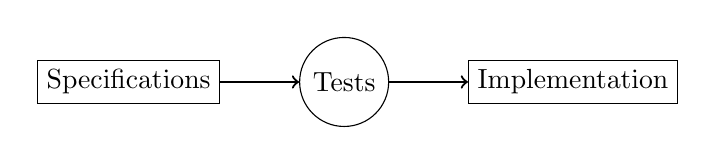
\begin{tikzpicture}
\matrix[column sep=10mm]{
    \node (id) [draw, shape=rectangle]{  Specifications  }; &
    \node (ts) [draw, shape=circle]   {  Tests  }; &
    \node (im) [draw, shape=rectangle]{  Implementation   };\\
};
\draw[->, thick] (id) -- (ts);
\draw[->, thick] (ts) -- (im);
\end{tikzpicture}
\end{center}

If the test cases are sufficiently thorough, when the tests all pass the program can be considered complete.
Remember, however, that it is not sufficient to just have tests, but to have tests that accurately and rigorously test the code.
To check that the test cases are sufficient, examine the test coverage and add additional tests if necessary.

% Kent Beck, the creator of \href{https://en.wikipedia.org/wiki/Extreme_programming}{extreme programming}, claims to have re-discovered TDD.
% He said,
% ``The original description of TDD was in an ancient book about programming.
% It said you take the input tape, manually type in the output tape you expect, then program until the actual output tape matches the expected output.''
% TDD eliminates the chore of testing code after it has been written.
% It also eliminates the fear that even though code is ``done,'' it may contain obscure bugs.
% Furthermore, writing unit tests helps the developer understand the project as a whole as well as the minute details of each piece.

See \url{https://en.wikipedia.org/wiki/Test-driven_development} for more discussion on TDD and \url{https://en.wikipedia.org/wiki/Behavior-driven_development} for an overview of Behavior-driven development (BDD), a close relative of TDD.

\begin{problem} % Write tests for Set.
\emph{Set} is a card game about finding patterns.
Each card contains a design with 4 different properties: color (red, green or purple), shape (diamond, oval or squiggly), quantity (one, two, or three) and pattern (solid, striped or outlined).
A \emph{set} is a group of three cards which are either all the same or all different for each property.
You can try playing Set online at \url{http://smart-games.org/en/set/start}.

Here is a group of twelve Set cards.
\begin{figure}[H]
    \centering
    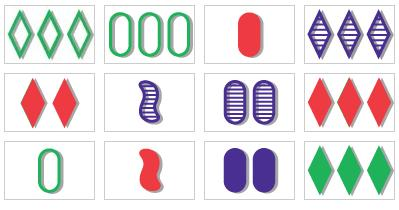
\includegraphics[width=.6\textwidth]{figures/set_game.jpg}
\end{figure}

This collection of cards contains six unique sets:
\begin{figure}[H] % Examples of sets.
\captionsetup[subfigure]{justification=centering}
\centering
\begin{subfigure}{.47\textwidth}
    \centering
    
\includegraphics[width=\linewidth]{figures/set1.jpg}
    \caption{Same in quantity and shape; different in pattern and color}
\end{subfigure}
%
\begin{subfigure}{.47\textwidth}
    \centering
    
\includegraphics[width=\linewidth]{figures/set6.jpg}
    \caption{Same in color and pattern; different in shape and quantity}
\end{subfigure}
\\
\begin{subfigure}{.47\textwidth}
    \centering
    
\includegraphics[width=\linewidth]{figures/set2.jpg}
    \caption{Same in pattern; different in shape, quantity and color}
\end{subfigure}
%
\begin{subfigure}{.47\textwidth}
    \centering
    
\includegraphics[width=\linewidth]{figures/set3.jpg}
    \caption{Same in shape; different in quantity, pattern and color}
\end{subfigure}
\\
\begin{subfigure}{.47\textwidth}
    \centering
    
\includegraphics[width=\linewidth]{figures/set4.jpg}
    \caption{Different in all aspects}
\end{subfigure}
%
\begin{subfigure}{.47\textwidth}
    \centering
    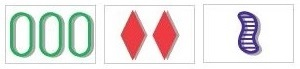
\includegraphics[width=\linewidth]{figures/set5.jpg}
    \caption{Different in all aspects}
\end{subfigure}
\end{figure}

Each Set card can be uniquely represented by a 4-bit integer in base 3,\footnote{A 4-bit integer in base 3 contains four digits that are either 0, 1 or 2. For example, 0000 and 1201 are 4-bit integers in base 3, whereas 000 is not because it has only three digits, and 0123 is not because it contains the number 3.} where each digit represents a different property and each property has three possible values.
A full hand in Set is a group of twelve unique cards, so a hand can be represented by a list of twelve 4-digit integers in base 3.
For example, the hand shown above could be represented by the following list.

\begin{lstlisting}
hand1 = ["1022", "1122", "0100", "2021",
         "0010", "2201", "2111", "0020",
         "1102", "0210", "2110", "1020"]
\end{lstlisting}

The following function definitions provide a framework for partially implementing Set by calculating the number of sets in a given hand. % (TDD step 1).

\newpage

\begin{lstlisting}
def count_sets(cards):
    """Return the number of sets in the provided Set hand.

    Parameters:
        cards (list(str)) a list of twelve cards as 4-bit integers in
        base 3 as strings, such as ["1022", "1122", ..., "1020"].
    Returns:
        (int) The number of sets in the hand.
    Raises:
        ValueError: if the list does not contain a valid Set hand, meaning
            - there are not exactly 12 cards,
            - the cards are not all unique,
            - one or more cards does not have exactly 4 digits, or
            - one or more cards has a character other than 0, 1, or 2.
    """
    pass

def is_set(a, b, c):
    """Determine if the cards a, b, and c constitute a set.

    Parameters:
        a, b, c (str): string representations of 4-bit integers in base 3.
            For example, "1022", "1122", and "1020" (which is not a set).
    Returns:
        True if a, b, and c form a set, meaning the ith digit of a, b,
            and c are either the same or all different for i=1,2,3,4.
        False if a, b, and c do not form a set.
    """
    pass
\end{lstlisting}

Write unit tests for these functions, but \textbf{do not} implement them yet.
Focus on \emph{what} the functions should do rather than on \emph{how} they will be implemented.
\\ (Hint: if three cards form a set, then the first digits of the cards are either all the same or all different.
Then the sums of these digits can only be 0, 3, or 6.
Thus a group of cards forms a set only if for each set of digits---first digits, second digits, etc.---the sum is a multiple of 3.)
\label{prob:tdd_tests}
\end{problem}

\begin{problem}
After you have written unit tests for the functions in Problem \ref{prob:tdd_tests}, implement the actual functions.
If needed, add additional test cases to get full coverage.
\\ (Hint: The \li{combinations()} function from the standard library module \li{itertools} may be useful in implementing \li{count_sets()}.)
\end{problem}

\newpage

\section*{Additional Material} % ==============================================

\subsection*{The Python Debugger} % -------------------------------------------

Python has a built in debugger called \li{pdb} to aid in finding mistakes in code during execution.
The debugger can be run either in a terminal or in a Jupyter Notebook.

A \emph{break point}, set with \li{pdb.set_trace()}, is a spot where the program pauses execution.
Once the program is paused, use the following commands to tell the program what to do next.

\begin{table}[H]
\centering
\begin{tabular}{r|l}
    Command & Description\\
    \hline
    \li{n} & \textbf{n}ext: executes the next line\\
    \li{p <var>} & \textbf{p}rint: display the value of the specified variable.\\
    \li{c} & \textbf{c}ontinue: stop debugging and run the program normally to the end.\\
    \li{q} & \textbf{q}uit: terminate the program.\\
    \li{l} & \textbf{l}ist: show several lines of code around the current line.\\
    \li{r} & \textbf{r}eturn: return to the end of a subroutine.\\
    \li{<Enter>} & Execute the most recent command again.
\end{tabular}
\end{table}

For example, suppose we have a long loop where the value of a variable changes unpredictably.

\begin{lstlisting}
# pdb_example.py
import pdb
from random import randint

i = 0
pdb.set_trace()                                     # Set a break point.
while i < 1000000000:
    i += randint(1, 10)
print("DONE")
\end{lstlisting}

Run the file in the terminal to begin a debugging session.

\begin{lstlisting}
$ python pdb_example.py
<<> /Users/Student/pdb_example.py(7)<module>()
-> while i < 1000000000:
(Pdb) l                                             >># Show where we are.
<<  2     import pdb
  3     from random import randint
  4
  5     i = 0
  6     pdb.set_trace()
  7  -> while i < 1000000000:
  8         i += randint(1, 10)
  9     print("DONE")
[EOF]>>
\end{lstlisting}

We can check the value of the variable \li{i} at any step with \li{p i}, and we can even change the value of \li{i} mid-program.

\begin{lstlisting}
(Pdb) n                                             # Execute a few lines.
> /Users/Student/pdb_example.py(8)<module>()
-> i += randint(1, 10)
(Pdb) n
> /Users/Student/pdb_example.py(7)<module>()
-> <<while>> i < 1000000000:
(Pdb) n
> /Users/Student/pdb_example.py(8)<module>()
-> i += randint(1, 10)
(Pdb) p i                                           # Check the value of i.
8
(Pdb) n                                             # Execute another line.
> /Users/Student/pdb_example.py(7)<module>()
-> <<while>> i < 1000000000:
(Pdb) p i                                           # Check i again.
14
(Pdb) i = 999999999                                 # Change the value of i.
(Pdb) c                                             # Continue the program.
DONE
\end{lstlisting}

See \url{https://docs.python.org/3/library/pdb.html} for documentation and examples for the Python debugger.

\subsection*{Other Testing Suites} % ------------------------------------------

There are several frameworks other than \li{pytest} for writing unit tests.
Each shares the same basic structure, but the setup, syntax, and particular features vary.
For more unit testing practice, try out the standard library's \li{unittest} (\url{https://docs.python.org/3/library/unittest.html}) or \li{doctest} (\url{https://docs.python.org/3/library/doctest.html}), or the third-party \li{nose} module (\url{https://nose.readthedocs.io/en/latest/}).
For a much larger list of unit testing tools, see \url{https://wiki.python.org/moin/PythonTestingToolsTaxonomy}.

\subsection*{The Fractions Module} % ------------------------------------------

The standard library's \li{fractions} module (\url{https://docs.python.org/3/library/fractions.html}) has a \li{Fraction} class that is similar to the \li{Fraction} class presented in this lab.
Its structure and syntax is a little different from this lab's class, but it is a little more robust in that it can take in floats, decimals, integers, and strings to its constructor.
See also the \li{decimals} module (\url{https://docs.python.org/3/library/decimal.html}) for tools relating to decimal arithmetic.
